
\noindent\begin{minipage}{\textwidth}
    \begin{table}[H]
        \centering
        \caption{Hiperparâmetros e Resultados do Melhor Modelo - resnet\_v1\_AB\_opt\_aug}
        \vspace{0.2cm}
        \resizebox{\textwidth}{!}{%
            \begin{tabular}{ll | lrrr}
                \hline
                \multicolumn{2}{c|}{\textbf{Hiperparâmetros}} & \multicolumn{4}{c}{\textbf{Métricas por Classe}} \\ \hline
                \textbf{Parâmetro} & \textbf{Valor} & \textbf{Classe} & \textbf{Precisão} & \textbf{Recall} & \textbf{F1-Score} \\ \hline
    Agendador de LR & StepLR & 31.2 & 0.5118 & 0.6726 & 0.5813 \\ 
Architecture & resnet34 & 31.3 & 0.5727 & 0.3119 & 0.4038 \\ 
Augmentation (Método) & None & 31.4 & 0.4488 & 0.4381 & 0.4434 \\ 
Batch Size & 32 & 32.3 & 0.6457 & 0.4184 & 0.5077 \\ 
Decaimento de Peso (WD) & 0.0003 & 32.4 & 0.5789 & 0.1897 & 0.2857 \\ 
Dropout & 0.5427 & 33.3 & 0.3689 & 0.6995 & 0.4830 \\ 
Função de Perda & CrossEntropyLoss & 41.4 & 0.5000 & 0.2727 & 0.3529 \\ 
Hidden Units & 512 & 41.5 & 0.4419 & 0.4872 & 0.4634 \\ 
Label Smoothing & 0.1000 & 42.4 & 0.4426 & 0.3971 & 0.4186 \\ 
Otimizador & AdamW & 44.4 & 0.7692 & 0.3448 & 0.4762 \\ 
\cline{3-6} 
Taxa de Aprendizado (LR) & 2.97e-04 & \textbf{Média (Macro)} & 0.5755 & 0.4417 & 0.4583 \\ 
Unfreeze Layers & 3 & \textbf{MCC} & \multicolumn{3}{c}{0.4160} \\ 
            \hline
            \end{tabular}%
        }
    \end{table}

    \begin{figure}[H]
        \centering
        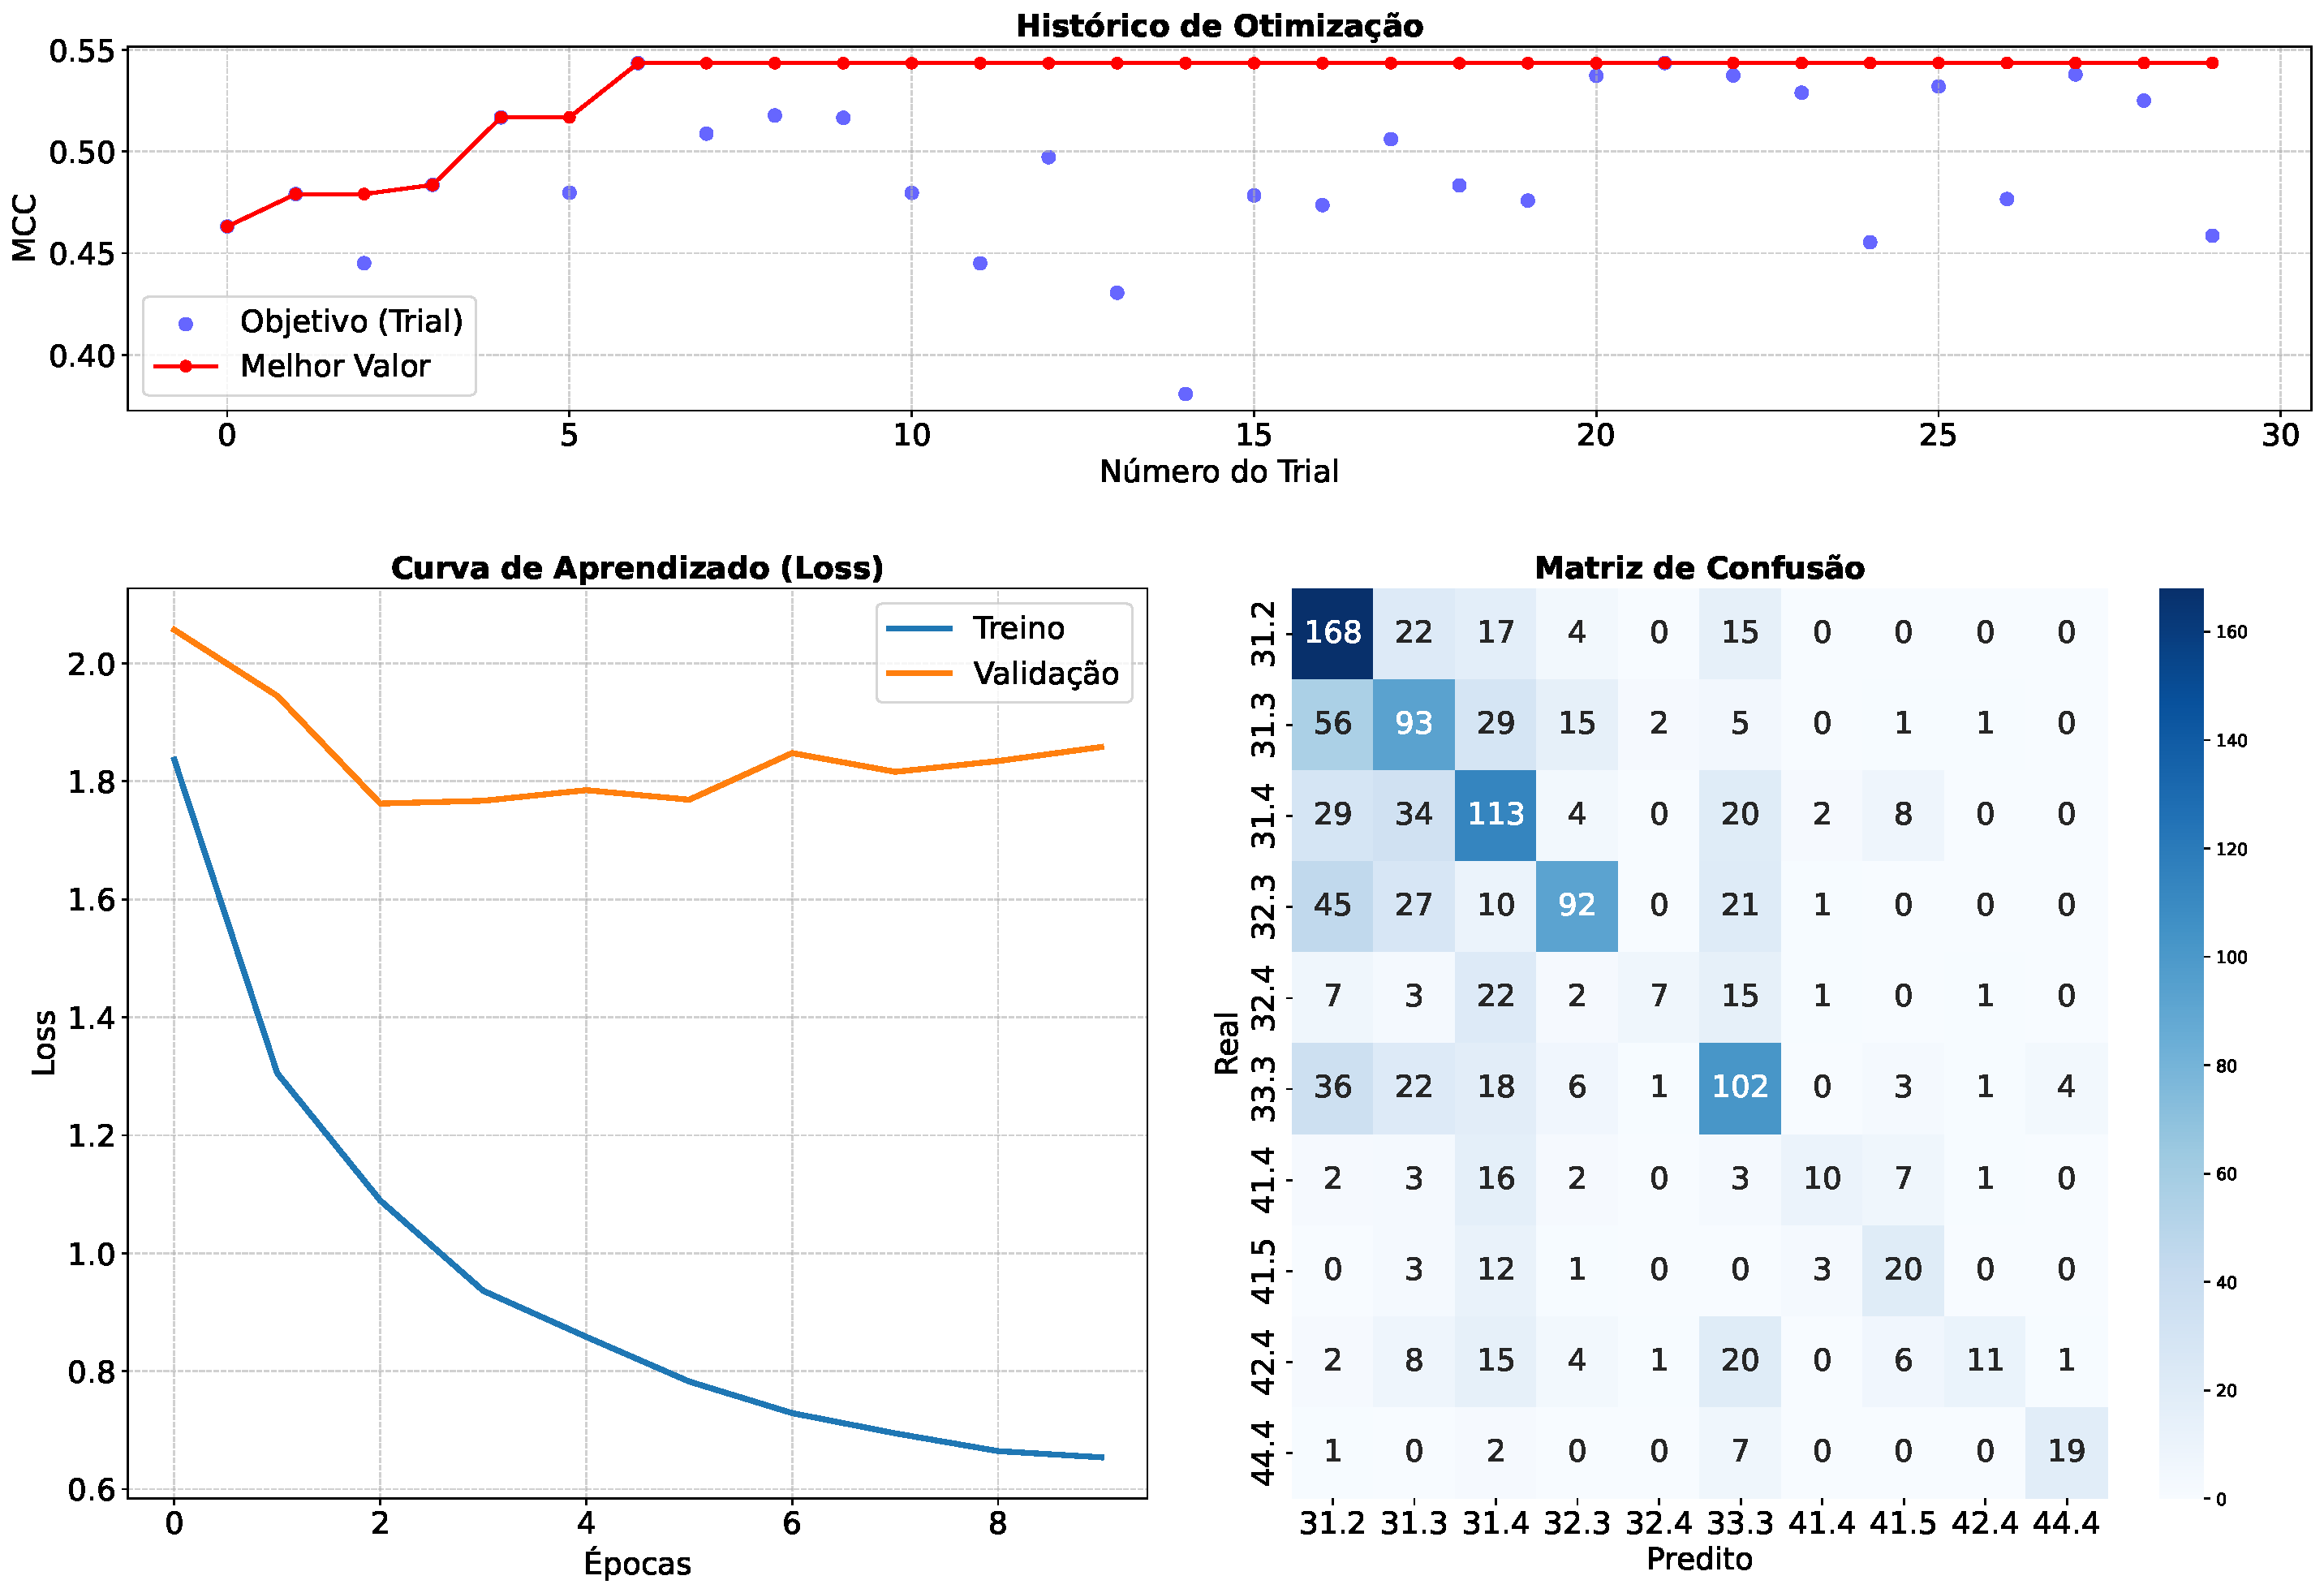
\includegraphics[width=0.85\textwidth]{tex/appendix/experiments/resnet_v1_AB_opt_aug/dashboard_consolidado.pdf}
        \caption{Histórico de Otimização, Curvas de Aprendizado e Matriz de Confusão - resnet\_v1\_AB\_opt\_aug}
    \end{figure}
\end{minipage}
\clearpage
